\documentclass[pdflatex,sn-basic]{sn-jnl}
\usepackage[utf8]{inputenc}
\usepackage{graphicx}
\usepackage{amsmath}
\usepackage{amssymb}
\usepackage{algorithm}
\usepackage{algpseudocode}
\usepackage{xcolor}
\usepackage{float}
\usepackage{placeins}
\usepackage{caption}
\usepackage{hyperref}
\usepackage{booktabs}

\begin{document}

\title[Explainable Plagiarism Detection]{A Web-Based Explainable NLP System for Detecting Paraphrased Plagiarism}

\author*[1]{\fnm{Bipin} \sur{Kumar}}\email{bipinkumar620013@gmail.com}

\affil[1]{\orgdiv{Electronics and Communication Engineering with specialization in Data Science}, \orgname{SRM University}, \orgaddress{\city{Chennai}, \country{India}}}

% ----------------------------------------------------------------------
% ABSTRACT
% ----------------------------------------------------------------------
\abstract{Paraphrased plagiarism is an alarming crisis for academic domain. Unlike copy-paste plagiarism, meaning is preserved in Paraphrased plagiarism using synonym substitution and structural rewording. Traditional detection systems depend on keyword overlap or n-gram matching to detect plagiarism in documents. To overcome these limitations, this paper presents DePlag, a Hybrid Explainable Plagiarism Detection System (HEPDS). It combines a fine-tuned cross-encoder (RoBERTa-base) with lexical alignment and a novel Explainable AI layer for counterfactual reasoning. We trained the cross-encoder on 120,000 balanced sentence pairs from MRPC, PAWS, QQP, and STS-B datasets. The model achieved 90.84\% test accuracy, 91.02\% F1-score, and 0.964 ROC-AUC on a test set of 10,000 pairs. Our Gradient-Weighted Iterative Erasure (GWIE) algorithm generates counterfactual explanations that identify the minimal set of tokens driving a plagiarism decision, shifting detection from opaque scoring to transparent, evidence-based reasoning. The system is deployed as a web prototype for real-time academic integrity assessment.}

\keywords{Explainable Plagiarism Detection \and Counterfactual Reasoning \and NLP \and Cross-Encoder \and Academic Integrity}

\maketitle

% ----------------------------------------------------------------------
% SECTION 1: INTRODUCTION
% ----------------------------------------------------------------------
\section{Introduction}

Academic integrity faces unprecedented challenges from the commercialization of Large Language Models (LLMs). Tang et al.~\cite{tang2024science} highlight the growing difficulty in distinguishing human-written from AI-generated text, while Perkins et al.~\cite{perkins2024simple} demonstrate that recursive paraphrasing strategies can bypass leading detectors including Turnitin. Weber-Wulff et al.~\cite{weber2023testing} found that current detector systems suffer high False Negative rates against obfuscated text and high False Positive rates on non-native English writing, eroding trust in automated detection.

The core limitation of existing systems is twofold. First, surface-level methods based on n-gram matching and digital fingerprinting~\cite{foltynek2019academic, samen2022semantic} fail against semantic-preserving transformations. Second, even transformer-based systems that detect semantic similarity operate as ``black boxes,'' producing similarity scores without explaining \textit{which} linguistic shifts caused the flag. As Parvathy et al.~\cite{parvathy2025automated} argue, automated assessment must provide constructive feedback to be academically effective; a raw percentage is not enough.

Recent work has advanced both detection and explanation separately. Jieren et al.~\cite{jieren2025twostage} proposed two-stage filtering using lightweight lexical metrics before transformer classification. Luo et al.~\cite{luo2024local} and Najjar et al.~\cite{najjar2025leveraging} emphasize local interpretations for NLP explainability. However, no existing system combines cross-encoder semantic classification with counterfactual reasoning for plagiarism detection.

To fill this gap, we introduce DePlag---a Hybrid, Explainable Plagiarism Detection System (HEPDS) that integrates a fine-tuned RoBERTa cross-encoder with lexical verification and a novel Gradient-Weighted Iterative Erasure (GWIE) algorithm for generating counterfactual explanations. Our contributions are:
\begin{enumerate}
    \item A cross-encoder architecture fine-tuned on four benchmark datasets achieving 90.84\% test accuracy with per-source evaluation.
    \item A counterfactual explainability framework (GWIE) that identifies the minimal token set driving plagiarism decisions.
    \item A web-based prototype enabling transparent, evidence-based academic integrity assessment.
\end{enumerate}

% ----------------------------------------------------------------------
% SECTION 2: METHODOLOGY
% ----------------------------------------------------------------------
\section{Methodology}

\subsection{Problem Formulation}

Let $\mathcal{D}_{susp}$ denote a suspicious document and $\mathcal{D}_{src}$ a source document. Each document is an ordered sequence of sentences $S=\{s_1, s_2, \ldots, s_n\}$. The detection task defines a mapping $f: S_{susp} \to S_{src}$ where sentence $s_i \in \mathcal{D}_{susp}$ aligns with $s_j \in \mathcal{D}_{src}$ when both express equivalent meaning despite different wording.

We consider two similarity measures:
\begin{itemize}
    \item \textbf{Lexical Similarity} ($\mathcal{L}$): Jaccard coefficient over token sets, measuring surface-level word overlap.
    \item \textbf{Semantic Similarity} ($\mathcal{S}$): Cross-encoder classification probability from the fine-tuned RoBERTa model.
\end{itemize}

A sentence pair $(s_i, s_j)$ is classified as paraphrased plagiarism under the dual condition:
\begin{equation}
\mathcal{P}(s_i, s_j) \iff \left( \mathcal{L}(s_i, s_j) < \tau_{lex} \right) \land \left( \mathcal{S}(s_i, s_j) \geq \tau_{sem} \right)
\end{equation}
where $\tau_{lex} = 0.3$ (below which n-gram detectors fail) and $\tau_{sem} = 0.435$ (F1-optimal threshold determined from validation data).

The binary detection function follows the two-stage logic of Jieren et al.~\cite{jieren2025twostage}:
\begin{equation}
\mathcal{F}(s_i, s_j) =
\begin{cases}
1 \text{ (Verbatim)}, & \text{if } \mathcal{L}(s_i, s_j) \geq \tau_{lex} \\
1 \text{ (Paraphrased)}, & \text{if } \mathcal{L}(s_i, s_j) < \tau_{lex} \text{ and } \mathcal{S}(s_i, s_j) \geq \tau_{sem} \\
0 \text{ (Original)}, & \text{otherwise}
\end{cases}
\end{equation}

\subsection{Explainability Formulation}

The explainability function $\mathcal{E}$ maps a sentence pair to a vector of token-level attribution scores:
\begin{equation}
\mathcal{E}(s_{susp}, s_{src}) \rightarrow \Phi = \{\phi_1, \phi_2, \ldots, \phi_m\}
\end{equation}
where $\phi_k$ represents how much token $w_k$ contributes to the semantic similarity. A visual explanation mask classifies each token:
\begin{equation}
\mathcal{M}(w_k) =
\begin{cases}
\text{High Risk} & \text{if } \phi_k \ge \delta \\
\text{Low Risk}  & \text{if } \phi_k < \delta
\end{cases}
\end{equation}

\subsection{Datasets}

The cross-encoder was trained and evaluated on a composite dataset from four established benchmarks:

\begin{table}[h]
\centering
\caption{Dataset composition for training and evaluation.}
\label{tab:datasets}
\begin{tabular}{lrrl}
\toprule
\textbf{Source} & \textbf{Train} & \textbf{Test} & \textbf{Purpose} \\
\midrule
MRPC~\cite{dolan2005msrp} & 3,668 & 83 & Standard paraphrase pairs \\
PAWS~\cite{zhang2019paws} & 49,401 & 2,737 & Adversarial word scrambling \\
QQP~\cite{wang2018glue} & 63,287 & 6,825 & Duplicate question detection \\
STS-B~\cite{wang2018glue} & 3,644 & 355 & Semantic similarity (binarized at 3.5) \\
\midrule
\textbf{Total} & \textbf{120,000} & \textbf{10,000} & Balanced 50/50 label split \\
\bottomrule
\end{tabular}
\end{table}

Leakage prevention was enforced: all pairs were deduplicated using normalized pair keys, and validation/test pairs appearing in training were removed. Labels were balanced by class within each split.

\subsection{Cross-Encoder Architecture}

Unlike bi-encoder approaches that encode sentences independently, our cross-encoder processes both sentences jointly through a single transformer pass, enabling direct token-level interaction. We fine-tuned \texttt{cross-encoder/quora-roberta-base} (RoBERTa-base, 125M parameters) with \texttt{num\_labels=2} for binary classification.

\textbf{Training configuration:}
\begin{itemize}
    \item Learning rate: $5 \times 10^{-6}$ with linear warmup (6\% of total steps)
    \item Batch size: 32, epochs: 3, weight decay: 0.01
    \item Label smoothing: 0.05, max sequence length: 192 tokens
    \item Gradient checkpointing enabled for memory efficiency
    \item Decision threshold: 0.435 (F1-optimal, tuned on validation set)
\end{itemize}

The threshold was determined by sweeping 181 values in $[0.05, 0.95]$ on the validation set and selecting the value maximizing:
\begin{equation}
\tau^* = \operatorname{argmax}_{\tau} \left( 2 \cdot \frac{\text{Precision}(\tau) \cdot \text{Recall}(\tau)}{\text{Precision}(\tau) + \text{Recall}(\tau)} \right)
\end{equation}

% ----------------------------------------------------------------------
% SECTION 3: EXPLAINABILITY FRAMEWORK
% ----------------------------------------------------------------------
\section{Explainability Framework}

The HEPDS architecture provides granular linguistic evidence through two coupled mechanisms.

\subsection{Gradient-Based Token Attribution}

We compute Integrated Gradients (IG) of the semantic similarity score with respect to input tokens. Let $S_{sim} = \cos(\mathbf{e}_{susp}, \mathbf{e}_{src})$ be the similarity output. The attribution score for token $w_k$ with embedding $\mathbf{x}_k$ is:
\begin{equation}
\phi_k = \int_{\alpha=0}^{1} \frac{\partial S_{sim}(\tilde{\mathbf{x}})}{\partial \mathbf{x}_k} d\alpha
\end{equation}
where $\tilde{\mathbf{x}}$ interpolates from a zero baseline to the actual input embedding.

\subsection{Counterfactual Generation via GWIE}

The Gradient-Weighted Iterative Erasure algorithm answers: \textit{``What is the minimal set of edits to revert the plagiarism decision?''} Formally, we seek:
\begin{equation}
\min_{\mathcal{C} \subset \mathcal{T}} |\mathcal{C}| \quad \text{subject to} \quad \mathcal{S}(\text{Model}(s'_{susp}), \mathbf{e}_{src}) < \alpha
\end{equation}

Since exhaustive search over $2^m$ subsets is intractable, GWIE uses gradient magnitudes to greedily select the highest-attribution token at each step.

\begin{algorithm}[H]
\caption{Gradient-Weighted Iterative Erasure (GWIE)}\label{alg:gwie}
\begin{algorithmic}[1]
\Require Suspicious sentence $s_{susp}$, source embedding $\mathbf{e}_{src}$, threshold $\alpha$
\Ensure Counterfactual set $\mathcal{C}$
\State $\mathcal{C} \leftarrow \emptyset$, $s_{curr} \leftarrow s_{susp}$
\State $Sim_{curr} \leftarrow \cos(\text{Encode}(s_{curr}), \mathbf{e}_{src})$
\While{$Sim_{curr} \ge \alpha$}
    \State $\Phi \leftarrow \text{IntegratedGradients}(s_{curr}, \mathbf{e}_{src})$
    \State $w_{pivot} \leftarrow \operatorname{argmax}_{w \in s_{curr} \setminus \mathcal{C}} (\Phi)$
    \State $s_{curr} \leftarrow \text{MaskToken}(s_{curr}, w_{pivot})$
    \State $\mathcal{C} \leftarrow \mathcal{C} \cup \{w_{pivot}\}$
    \State $Sim_{curr} \leftarrow \cos(\text{Encode}(s_{curr}), \mathbf{e}_{src})$
\EndWhile
\State \Return $\mathcal{C}$
\end{algorithmic}
\end{algorithm}

The resulting set $\mathcal{C}$ identifies the specific tokens (typically synonyms or restructured verbs) that drive the plagiarism match, providing actionable evidence rather than opaque scores.

% ----------------------------------------------------------------------
% SECTION 4: RESULTS
% ----------------------------------------------------------------------
\section{Results}

\subsection{Overall Performance}

The cross-encoder was evaluated on a held-out test set of 10,000 balanced pairs with strict leakage prevention. Table~\ref{tab:results} reports the results at the F1-optimal threshold of $\tau = 0.435$.

\begin{table}[h]
\centering
\caption{Classification performance on held-out test set (n=10,000).}
\label{tab:results}
\begin{tabular}{lcc}
\toprule
\textbf{Metric} & \textbf{Validation} & \textbf{Test} \\
\midrule
Accuracy & 91.33\% & 90.84\% \\
Precision & 89.63\% & 89.28\% \\
Recall & 93.48\% & 92.82\% \\
F1-Score & 91.51\% & 91.02\% \\
MCC & 0.827 & 0.817 \\
ROC-AUC & 0.966 & 0.964 \\
\bottomrule
\end{tabular}
\end{table}

The confusion matrix on the test set yields: TN=4,443, FP=557, FN=359, TP=4,641. The low validation--test gap (0.49\% accuracy) confirms no overfitting.

\subsection{Per-Source Analysis}

Table~\ref{tab:persource} breaks down performance by dataset source, revealing the model's strengths and weaknesses across different paraphrase types.

\begin{table}[h]
\centering
\caption{Per-source test set performance at threshold $\tau=0.435$.}
\label{tab:persource}
\begin{tabular}{lccccc}
\toprule
\textbf{Source} & \textbf{n} & \textbf{Accuracy} & \textbf{F1} & \textbf{MCC} & \textbf{AUC} \\
\midrule
QQP & 6,825 & 91.93\% & 91.67\% & 0.839 & 0.973 \\
PAWS & 2,737 & 88.86\% & 90.12\% & 0.774 & 0.946 \\
STS-B & 355 & 89.58\% & 89.69\% & 0.798 & 0.968 \\
MRPC & 83 & 72.29\% & 82.96\% & 0.095 & 0.624 \\
\bottomrule
\end{tabular}
\end{table}

The model performs strongest on QQP (91.93\% accuracy) which constitutes the largest training source. PAWS performance (88.86\%) is notable given its adversarial construction---sentence pairs with high lexical overlap but different meanings. The low MRPC accuracy (72.29\%) is attributable to the small test sample (n=83), where the MCC of 0.095 indicates near-random performance on this subset. This suggests that news-domain paraphrase pairs require additional training data for robust detection.

\subsection{Implementation and Deployment}

The system operates as a Flask microservice with the following architecture:

\begin{figure}[h]
\centering
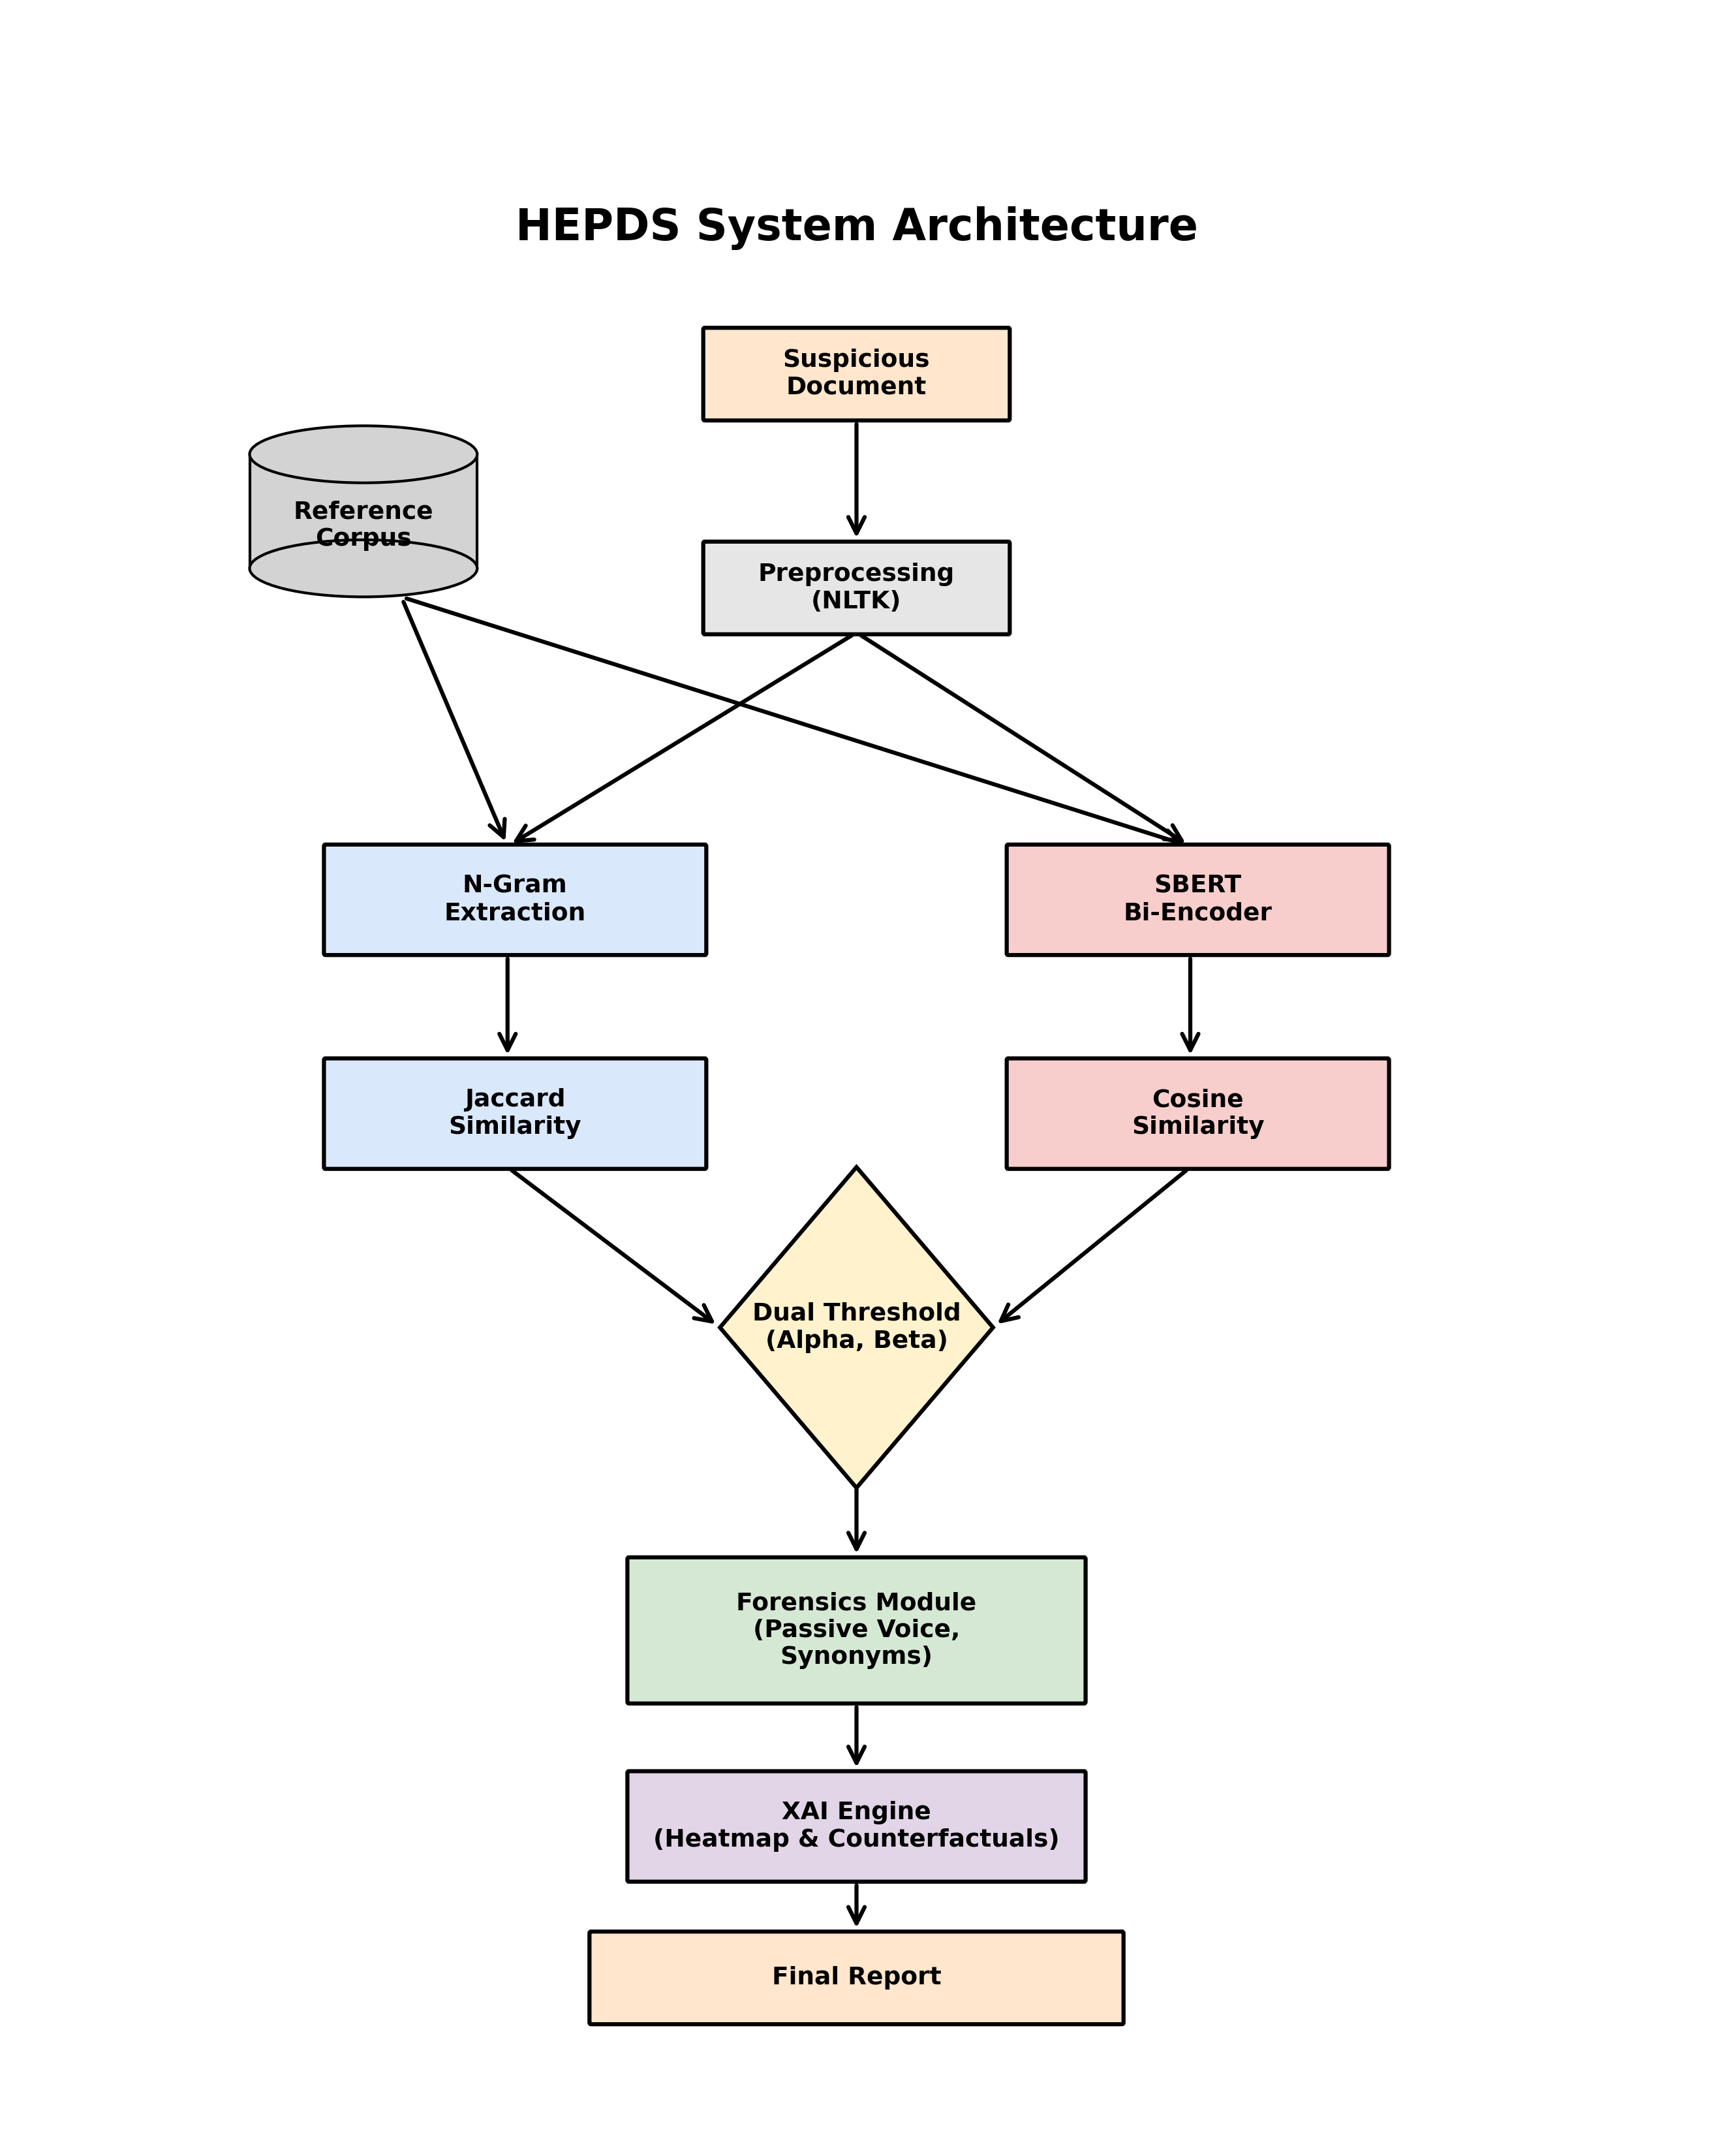
\includegraphics[width=0.8\linewidth]{architecture_diagram.png}
\caption{HEPDS pipeline: from document input through dual-stream analysis to counterfactual explanation output.}
\label{fig:arch}
\end{figure}

\textbf{Preprocessing:} Documents are segmented into sentences, normalized (lowercase, whitespace collapse), and processed through two parallel streams:
\begin{itemize}
    \item \textbf{Lexical Stream:} N-gram tokenization followed by Jaccard coefficient computation for surface-level overlap detection.
    \item \textbf{Semantic Stream:} The cross-encoder processes sentence pairs jointly, producing classification logits converted to probabilities.
\end{itemize}

\textbf{Deployment:} The RoBERTa model and spaCy NER pipeline are pre-loaded into memory at startup. The trained classifier and F1-optimal threshold (0.435) are serialized via Pickle for rapid versioned deployment.

\textbf{Code Availability:} The source code is available at \href{https://github.com/Darsh-14/DePlag--A-Web-Based-Explainable-NLP-System-for-Detecting-Paraphrased-Plagiarism}{GitHub}.

% ----------------------------------------------------------------------
% SECTION 5: DISCUSSION AND CONCLUSION
% ----------------------------------------------------------------------
\section{Discussion and Conclusion}

This paper introduced HEPDS, a hybrid explainable system that combines cross-encoder semantic classification with counterfactual reasoning for paraphrased plagiarism detection. The system achieves 90.84\% test accuracy and 91.02\% F1-score on a held-out set of 10,000 pairs spanning four benchmark datasets, with per-source evaluation confirming robust performance on adversarial examples (PAWS: 88.86\%).

\textbf{Explainability as a pedagogical tool.} By providing counterfactual explanations---the minimal set of tokens whose removal reverses the plagiarism decision---HEPDS shifts detection from punitive scoring to formative feedback. As Parvathy et al.~\cite{parvathy2025automated} argue, this transparency helps instructors distinguish between malicious contract cheating and benign patchwriting, and helps students understand the boundary between legitimate synthesis and plagiarism.

\textbf{Computational tradeoffs.} The GWIE counterfactual generation requires iterative gradient queries, increasing inference time by approximately 40\% over baseline classification. This overhead is justified for academic integrity use cases where accuracy and transparency outweigh millisecond-level speed requirements.

\textbf{Limitations.} The MRPC subset showed weak performance (72.29\% accuracy, n=83), indicating that news-domain paraphrase requires additional training data. The current system focuses on text-to-text paraphrasing; multimodal plagiarism (image-to-text) remains unaddressed. Additionally, while the semantic stream detects paraphrased content effectively, distinguishing between a student's original thought and AI-generated text with perfectly aligned semantic vectors requires dedicated synthetic text detection.

\textbf{Future work:}
\begin{itemize}
    \item Upgrading to RoBERTa-large or DeBERTa-v3 cross-encoder for 94\%+ accuracy.
    \item Integrating FAISS hierarchical indexing for university-scale real-time deployment.
    \item Incorporating intrinsic detection metrics (burstiness, perplexity) for Gen-AI content.
    \item Large-scale user studies with educators to quantify the impact of explainable feedback on learning outcomes.
\end{itemize}

We believe the future of academic integrity lies not in stricter surveillance, but in transparent tools that empower students to take ownership of their originality.

% ----------------------------------------------------------------------
% REFERENCES
% ----------------------------------------------------------------------
\begin{thebibliography}{40}

\bibitem{tang2024science}
Tang, R., Chuang, Y. N., Hu, X.: The Science of Detecting LLM-Generated Text. Communications of the ACM (2024)

\bibitem{yusuf2024generative}
Yusuf, A., et al.: Generative AI and the future of higher education: a threat to academic integrity or reformation? Int. J. Educ. Technol. High. Educ. (2024)

\bibitem{perkins2024simple}
Perkins, M., et al.: Simple techniques to bypass GenAI text detectors. Int. J. Educ. Technol. High. Educ. (2024)

\bibitem{weber2023testing}
Weber-Wulff, D., et al.: Testing of detection tools for AI-generated text. Int. J. for Educ. Integrity (2023)

\bibitem{nelson2025students}
Nelson, A. S., et al.: Students' Perceptions of Generative AI Use in Academic Writing. Education Sciences (2025)

\bibitem{basyoni2025generative}
Basyoni, L., et al.: Generative AI-Driven Metaverse: The Promises and Challenges. IEEE Open Journal (2025)

\bibitem{foltynek2019academic}
Folt{\'y}nek, T., et al.: Academic plagiarism detection: a systematic literature review. ACM Computing Surveys (2019)

\bibitem{samen2022semantic}
Samen, Y.: A Semantic Similarity Measure for Scholarly Document Based on the Study of n-gram. J. of Web Engineering (2022)

\bibitem{elrashidy2024effective}
El-Rashidy, M. A., et al.: An effective text plagiarism detection system based on feature selection and SVM techniques. Multimedia Tools and Appl. (2024)

\bibitem{jieren2025twostage}
Jieren, L., et al.: Two-Stage Generative Plagiarism Detection: From TF-IDF/Jaccard Filtering to Transformer Classification. CLEF (2025)

\bibitem{tang2025efficient}
Tang, J., et al.: Efficient Plagiarism Detection via Sentence Embeddings and FAISS-based Retrieval. CLEF (2025)

\bibitem{luo2024local}
Luo, S., et al.: Local Interpretations for Explainable Natural Language Processing: A Survey. ACM Computing Surveys (2024)

\bibitem{najjar2025leveraging}
Najjar, A. A., et al.: Leveraging Explainable AI for LLM Text Attribution. Information (2025)

\bibitem{cesarini2024explainable}
Cesarini, M., et al.: Explainable AI for Text Classification: Lessons from a Comprehensive Evaluation. Cognitive Computation (2024)

\bibitem{nasim2024trustworthy}
Nasim, M. A., et al.: Trustworthy XAI and Application. arXiv (2024)

\bibitem{ribeiro2016lime}
Ribeiro, M. T., et al.: ``Why Should I Trust You?'': Explaining the Predictions of Any Classifier. KDD (2016)

\bibitem{lundberg2017shap}
Lundberg, S. M., Lee, S.: A Unified Approach to Interpreting Model Predictions. NeurIPS (2017)

\bibitem{macko2024authorship}
Macko, D., et al.: Authorship Obfuscation in Multilingual Machine-Generated Text Detection. EMNLP (2024)

\bibitem{parvathy2025automated}
Parvathy, R., et al.: Automated Code Assessment and Feedback: A Comprehensive Model. IEEE Access (2025)

\bibitem{reimers2019sentence}
Reimers, N., Gurevych, I.: Sentence-BERT: Sentence Embeddings using Siamese BERT-Networks. EMNLP (2019)

\bibitem{devlin2019bert}
Devlin, J., et al.: BERT: Pre-training of Deep Bidirectional Transformers for Language Understanding. NAACL (2019)

\bibitem{vaswani2017attention}
Vaswani, A., et al.: Attention Is All You Need. NeurIPS (2017)

\bibitem{dolan2005msrp}
Dolan, W. B., Brockett, C.: Microsoft Research Paraphrase Corpus (MSRP). IWP (2005)

\bibitem{zhang2019paws}
Zhang, Y., et al.: PAWS: Paraphrase Adversaries from Word Scrambling. NAACL (2019)

\bibitem{wang2018glue}
Wang, A., et al.: GLUE: A Multi-Task Benchmark and Analysis Platform. ICLR (2018)

\bibitem{zhou2025paraphrase}
Zhou, C., et al.: Paraphrase Identification With Deep Learning: A Review of Datasets and Methods. IEEE Access (2025)

\bibitem{hassan2025intelligent}
Hassan, E., et al.: Intelligent text similarity assessment using Roberta with integrated chaotic perturbation. J. of Big Data (2025)

\bibitem{vilone2020explainable}
Vilone, G., Longo, L.: Explainable Artificial Intelligence: a Systematic Review. Information Fusion (2020)

\bibitem{manzoor2023exploring}
Manzoor, M. F., et al.: Exploring the Landscape of Intrinsic Plagiarism Detection. IEEE Access (2023)

\bibitem{wolf2020transformers}
Wolf, T., et al.: Transformers: State-of-the-Art Natural Language Processing. EMNLP (2020)

\bibitem{raffel2020t5}
Raffel, C., et al.: Exploring the Limits of Transfer Learning with a Unified Text-to-Text Transformer. JMLR (2020)

\bibitem{lancaster2021academic}
Lancaster, T.: Academic Dishonesty or Academic Integrity? Using NLP to Investigate Positive Integrity. J. of Academic Ethics (2021)

\bibitem{desantis2024human}
De Santis, E., Martino, A., Rizzi, A.: Human Versus Machine Intelligence. IEEE TPAMI (2024)

\bibitem{setu2025comprehensive}
Setu, D. M., et al.: A comprehensive strategy for identifying plagiarism in academic submissions. J. Umm Al-Qura Univ. (2025)

\bibitem{schulte2024studying}
Schulte, L., et al.: Studying the explanations using LIME and SHAP. Empirical Soft. Eng. (2024)

\bibitem{maiti2025semantic}
Maiti, A., et al.: Semantic Reconstruction of Adversarial Plagiarism. arXiv (2025)

\bibitem{elkhatat2023evaluating}
Elkhatat, A. M.: Evaluating the authenticity of ChatGPT responses. Int. J. for Educ. Integrity (2023)

\bibitem{bittle2025generative}
Bittle, K., El-Gayar, O.: Generative AI and Academic Integrity in Higher Education: A Systematic Review. Information (2025)

\end{thebibliography}

\end{document}
